\documentclass[border=4pt,12pt]{standalone}
% House style for redrawn exam diagrams (diagram-v4: 0.4pt lines, filled -latex arrows, fine dashes; stipple and hatching drawn as real dots/lines (no PDF/SVG patterns, so they render in every browser and at any scale); transparent background). Every figure \input's this.
\usepackage{amsmath,amssymb}
\usepackage{txfonts}
\usepackage{pdfrender,xcolor}
% \halo{text}: label on shading. The shading stops just around each letter's outline (a thin knock-out that follows the
% glyphs, like the papers' typesetting), never a box. Owner: "I don't want a box around the text".
\newcommand{\halo}[1]{\leavevmode\rlap{\pdfrender{TextRenderingMode=2,LineWidth=2.2pt,LineJoinStyle=1,StrokeColor=white,FillColor=white}#1}#1}
\usepackage{tikz,pgfplots}
\pgfplotsset{compat=1.18}
\usetikzlibrary{arrows.meta,calc,angles,quotes,patterns,patterns.meta,intersections,positioning,decorations.markings,shapes.geometric}
% Stipple and hatching are drawn as actual dots / lines clipped to the region (path picture), NOT as pattern fills:
% SVG <pattern> fills vanish or blur when browsers scale the image, so the owner could not see the shading.
% Each dot is a 0.72pt square (keeps SVGs small; reads as a dot at print size). Dots sit on one global staggered grid, so neighbouring regions line up.
\makeatletter
\newdimen\ex@x \newdimen\ex@y \newdimen\ex@xa \newdimen\ex@ya \newdimen\ex@xb \newdimen\ex@yb \newcount\ex@row
\def\exam@stipplecolor{black!75}\def\exam@dotr{0.42pt}\def\exam@dotgap{2.5}
\def\ex@rowdots{\ifdim\ex@x<\ex@xb \pgfpathrectangle{\pgfqpoint{\dimexpr\ex@x-0.36pt\relax}{\dimexpr\ex@y-0.36pt\relax}}{\pgfqpoint{0.72pt}{0.72pt}}\advance\ex@x by \exam@dotgap pt\relax\expandafter\ex@rowdots\fi}
\def\exam@stipple{%
  \pgftransformreset% dots are sized in real points even inside scaled pictures
  \pgfpointanchor{path picture bounding box}{south west}\ex@xa=\pgf@x \ex@ya=\pgf@y
  \pgfpointanchor{path picture bounding box}{north east}\ex@xb=\pgf@x \ex@yb=\pgf@y
  \pgfsetfillcolor{\exam@stipplecolor}\pgfmathsetmacro\ex@h{\exam@dotgap/2}%
  \pgfmathtruncatemacro\ex@r{floor(\ex@ya/\ex@h)-1}\ex@row=\ex@r\relax
  \ex@y=\ex@r\dimexpr\ex@h pt\relax
  \loop\ifdim\ex@y<\ex@yb
    \pgfmathtruncatemacro\ex@c{floor(\ex@xa/\exam@dotgap)-1}\ex@x=\ex@c\dimexpr\exam@dotgap pt\relax
    \ifodd\ex@row \advance\ex@x by \ex@h pt\fi
    \ex@rowdots
    \advance\ex@y by \ex@h pt \advance\ex@row by 1
    \ifnum\numexpr\ex@row-(\ex@row/4)*4\relax=0 \pgfusepath{fill}\fi% flush every 4 rows: bounded TeX memory, few clip copies in the SVG
  \repeat\pgfusepath{fill}}
\newdimen\ex@d
\def\exam@hatch#1{% #1 = 1 for /, -1 for \ ; lines 45 degrees, 3pt apart
  \pgftransformreset
  \pgfpointanchor{path picture bounding box}{south west}\ex@xa=\pgf@x \ex@ya=\pgf@y
  \pgfpointanchor{path picture bounding box}{north east}\ex@xb=\pgf@x \ex@yb=\pgf@y
  \ex@d=\dimexpr\ex@yb-\ex@ya\relax \ex@x=\dimexpr\ex@xa-\ex@d\relax
  \loop\ifdim\ex@x<\ex@xb
    \ifnum#1>0 \pgfpathmoveto{\pgfqpoint{\ex@x}{\ex@ya}}\pgfpathlineto{\pgfqpoint{\dimexpr\ex@x+\ex@d\relax}{\ex@yb}}%
    \else \pgfpathmoveto{\pgfqpoint{\ex@x}{\ex@yb}}\pgfpathlineto{\pgfqpoint{\dimexpr\ex@x+\ex@d\relax}{\ex@ya}}\fi
    \advance\ex@x by 4.24pt
  \repeat
  \pgfsetlinewidth{0.4pt}\pgfsetstrokecolor{black}\pgfusepath{stroke}}
\def\examstipple{\exam@stipple}\def\examhatch{\exam@hatch}\def\examsetstipplecolor#1{\def\exam@stipplecolor{#1}}\def\examsetdotgap#1{\def\exam@dotgap{#1}}
\makeatother
% (legacy pattern kept for old files)
% staggered stipple like the NESA papers' dotted shading
\pgfdeclarepatternformonly{exam stipple}{\pgfpointorigin}{\pgfqpoint{2.2pt}{2.2pt}}{\pgfqpoint{2.2pt}{2.2pt}}{%
  \pgfpathcircle{\pgfqpoint{0.55pt}{0.55pt}}{0.42pt}\pgfpathcircle{\pgfqpoint{1.65pt}{1.65pt}}{0.42pt}\pgfusepath{fill}}
\tikzset{
  every picture/.style={line width=0.6pt, >={Latex[length=2mm,width=1.3mm]}},
  curve/.style={line width=0.6pt},
  open arrow/.style={-{Latex[length=2mm,width=1.3mm]}},  % owner: filled -latex heads everywhere, no open chevrons
  aux/.style={dash pattern=on 2pt off 1.5pt, line width=0.6pt},
  shade/.code={\def\exA{#1}\def\exB{none}\ifx\exA\exB\else\pgfkeysalso{fill=black!18}\fi},
  shade/.default=on,
  shade dots/.style={fill=none, path picture={\examstipple}},
  stipple color/.code={\examsetstipplecolor{#1}},
  stipple gap/.code={\examsetdotgap{#1}},
  shade dense dots/.style={fill=none, stipple gap=1.6, path picture={\examstipple}},
  shade hatch/.style={fill=none, path picture={\examhatch{1}}},
  shade hatch reverse/.style={fill=none, path picture={\examhatch{-1}}},
  shade solid/.style={fill=black},
  pt/.style={circle, fill, inner sep=1.1pt},
  open pt/.style={circle, draw, fill=white, inner sep=1.1pt},
}
\pgfplotsset{
  exam axes/.style={axis lines=middle, axis line style={->}, xlabel={$x$}, ylabel={$y$},
    xlabel style={anchor=west}, ylabel style={anchor=south}, tick label style={font=\small},
    every axis plot/.append style={line width=0.6pt, black}, samples=200, clip=false,
    enlargelimits=false, axis on top},
}

\begin{document}
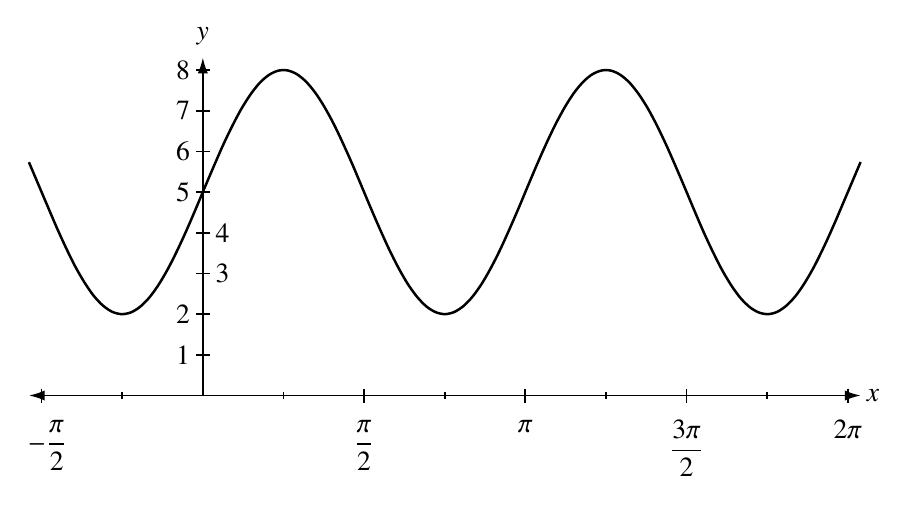
\begin{tikzpicture}[x=0.0127cm, y=-0.0127cm]
  \draw[smooth,line width=0.9pt] plot coordinates {(81.0,140.6) (90.2,162.3) (99.5,184.2) (108.7,205.7) (118.0,226.1) (127.2,244.7) (136.5,260.8) (145.7,274.1) (155.0,284.0) (164.2,290.2) (173.4,292.6) (182.7,291.0) (191.9,285.5) (201.2,276.3) (210.4,263.7) (219.7,248.0) (228.9,229.9) (238.2,209.8) (247.4,188.5) (256.6,166.6) (265.9,144.8) (275.1,123.8) (284.4,104.4) (293.6,87.1) (302.9,72.5) (312.1,61.0) (321.4,53.1) (330.6,49.0) (339.8,48.8) (349.1,52.6) (358.3,60.1) (367.6,71.3) (376.8,85.6) (386.1,102.7) (395.3,122.0) (404.6,142.8) (413.8,164.6) (423.0,186.5) (432.3,207.9) (441.5,228.1) (450.8,246.5) (460.0,262.4) (469.3,275.3) (478.5,284.8) (487.8,290.6) (497.0,292.6) (506.2,290.6) (515.5,284.7) (524.7,275.2) (534.0,262.2) (543.2,246.3) (552.5,227.9) (561.7,207.7) (571.0,186.3) (580.2,164.3) (589.4,142.6) (598.7,121.7) (607.9,102.5) (617.2,85.4) (626.4,71.1) (635.7,60.0) (644.9,52.5) (654.2,48.8) (663.4,49.0) (672.6,53.2) (681.9,61.1) (691.1,72.6) (700.4,87.2) (709.6,104.6) (718.9,124.1) (728.1,145.0) (737.4,166.8) (746.6,188.7) (755.8,210.1) (765.1,230.1) (774.3,248.2) (783.6,263.8) (792.8,276.4) (802.1,285.6) (811.3,291.0) (820.6,292.6) (829.8,290.2) (839.0,283.9) (848.3,274.0) (857.5,260.7) (866.8,244.5) (876.0,225.9) (885.3,205.5) (894.5,184.0) (903.8,162.1) (913.0,140.4)};
  \draw[<->] (81,374) -- (913,374);
  \draw[->] (255,374) -- (255,36);
  \node[anchor=west,inner sep=0] at (917,374) {$x$};
  \node[anchor=center,inner sep=0] at (255,15) {$y$};
  \draw (248,333.3) -- (262,333.3); \node[anchor=east,inner sep=0] at (243,333.3) {$1$};
  \draw (248,292.6) -- (262,292.6); \node[anchor=east,inner sep=0] at (243,292.6) {$2$};
  \draw (248,251.9) -- (262,251.9); \node[anchor=west,inner sep=0] at (267,251.9) {$3$};
  \draw (248,211.2) -- (262,211.2); \node[anchor=west,inner sep=0] at (267,211.2) {$4$};
  \draw (248,170.5) -- (262,170.5); \node[anchor=east,inner sep=0] at (243,170.5) {$5$};
  \draw (248,129.8) -- (262,129.8); \node[anchor=east,inner sep=0] at (243,129.8) {$6$};
  \draw (248,89.1) -- (262,89.1); \node[anchor=east,inner sep=0] at (243,89.1) {$7$};
  \draw (248,48.4) -- (262,48.4); \node[anchor=east,inner sep=0] at (243,48.4) {$8$};
  \draw (93.7,367) -- (93.7,381);
  \draw (174.3,370.5) -- (174.3,377.5);
  \draw (335.6,370.5) -- (335.6,377.5);
  \draw (416.3,367) -- (416.3,381);
  \draw (497.0,370.5) -- (497.0,377.5);
  \draw (577.6,367) -- (577.6,381);
  \draw (658.2,370.5) -- (658.2,377.5);
  \draw (738.9,367) -- (738.9,381);
  \draw (819.6,370.5) -- (819.6,377.5);
  \draw (900.2,367) -- (900.2,381);
  \node[anchor=north,inner sep=0] at (100,398) {$-\dfrac{\pi}{2}$};
  \node[anchor=north,inner sep=0] at (416.3,398) {$\dfrac{\pi}{2}$};
  \node[anchor=north,inner sep=0] at (577.6,398) {$\pi$};
  \node[anchor=north,inner sep=0] at (738.9,398) {$\dfrac{3\pi}{2}$};
  \node[anchor=north,inner sep=0] at (900.2,398) {$2\pi$};
\end{tikzpicture}
\end{document}
